%!TEX root = ../../Main.tex

\subsection{Задача 1}

Розглянемо задачу

\begin{equation}\label{eq:problem1}
\begin{split}
	- \Delta u(x_1,x_2) + 1000u(x_1, x_2) = f(x,y) \\
	f(x,y) = (18 \pi^2 +1000)\sin(3 \pi x) \sin (3 \pi y) \\
	u|_\Gamma = 0 \\
	\Gamma = \left[0;1\right] \times \left[0;1\right]
\end{split}
\end{equation}

її точний розв'язок

\begin{equation}
	u(x,y) = \sin(3 \pi x) \sin (3 \pi y)
\end{equation}

вигляд якого зображений на \autoref{plot:problem1_exact}

\begin{figure}[H]
	\centering
    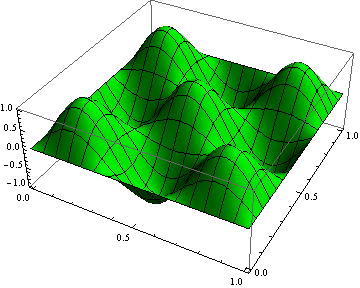
\includegraphics[scale=1.0]{problem1/ExactSolution}
    \caption{Точний розв'язок задачі \eqref{eq:problem1}}
    \label{plot:problem1_exact}
\end{figure}

Для апроксимації задамо граничну точність в 5\%.
В якості початкового розбиття виберемо рівномірне на сітці 10x10 (\autoref{fig:init_mesh1}).

\begin{figure}[H]
	\centering
    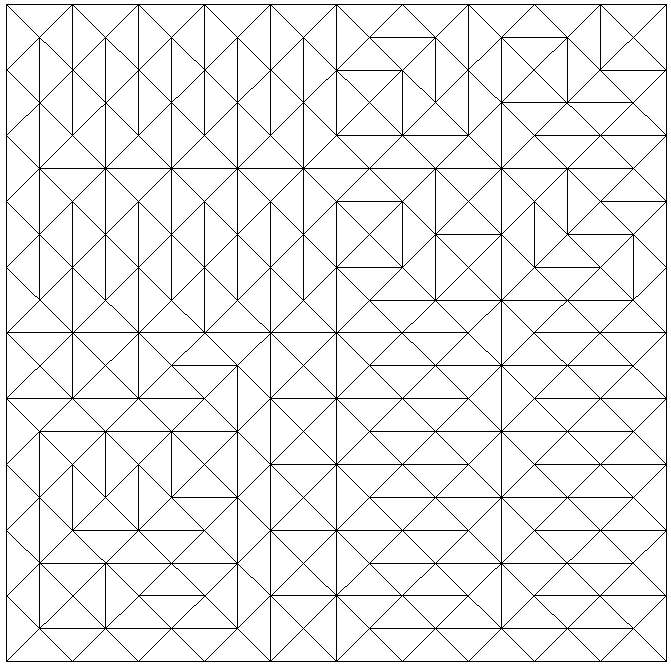
\includegraphics[scale=0.7]{problem1/InitialMesh}
    \caption{Початкове розбиття схеми}
    \label{fig:init_mesh1}
\end{figure}


Графіки обчисленого наближення зображені на \autoref{fig:p1_solution1}-\ref{fig:p1_solution18}


\begin{figure}[H]
	\centering
    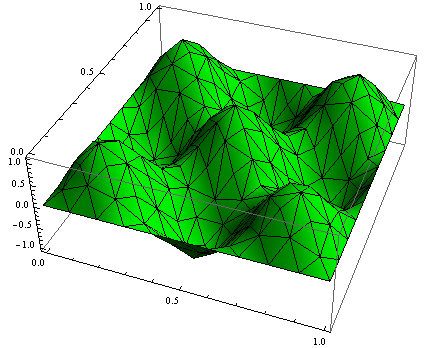
\includegraphics[scale=0.9]{problem1/my/solutions/1}
    \caption{Перша ітерація. Кількість скінченних елементів - 400}
    \label{fig:p1_solution1}
\end{figure}

\begin{figure}[H]
	\centering
    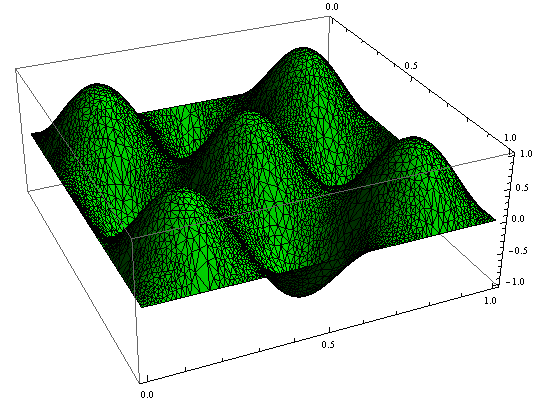
\includegraphics[scale=0.7]{problem1/my/solutions/5}
    \caption{5-та ітерація. Кількість скінченних елементів - 12903}
    \label{fig:p1_solution5}
\end{figure}

\begin{figure}[H]
	\centering
    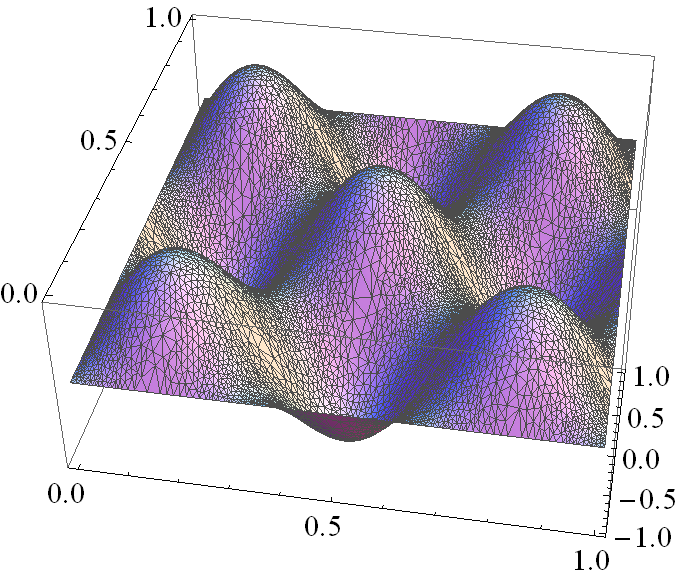
\includegraphics[scale=0.7]{problem1/my/solutions/18}
    \caption{18-та ітерація. Кількість скінченних елементів - 19322}
    \label{fig:p1_solution18}
\end{figure}

Графіки індикаторів похибок на скінченних елементах.

\begin{figure}[H]
	\centering
    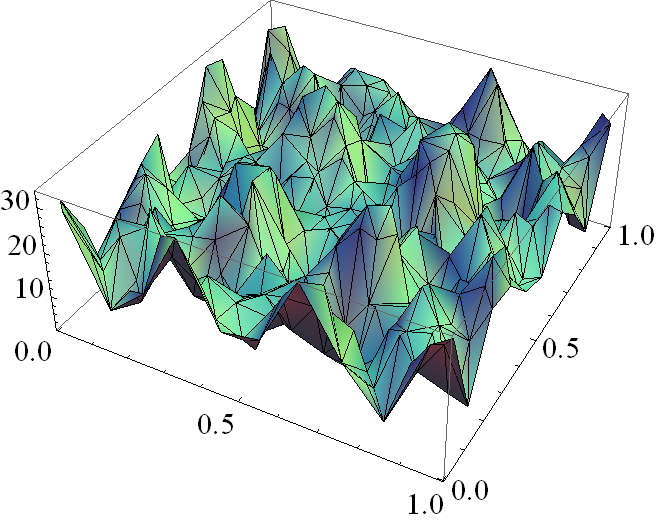
\includegraphics[scale=0.8]{problem1/my/AEE/1}
    \caption{Перша ітерація. Кількість скінченних елементів - 400}
    \label{fig:p1_aee1}
\end{figure}

\begin{figure}[H]
	\centering
    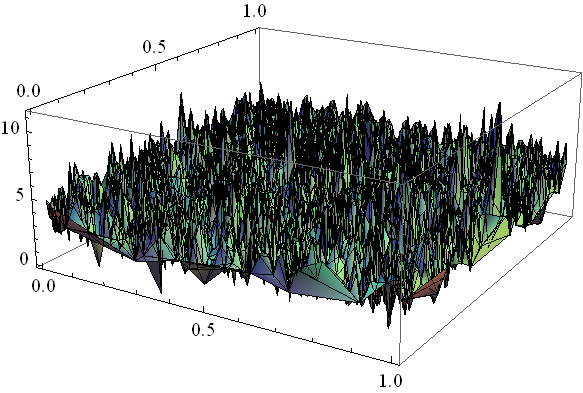
\includegraphics[scale=0.85]{problem1/my/AEE/5}
    \caption{5-та ітерація. Кількість скінченних елементів - 12903}
    \label{fig:p1_aee5}
\end{figure}

\begin{figure}[H]
	\centering
    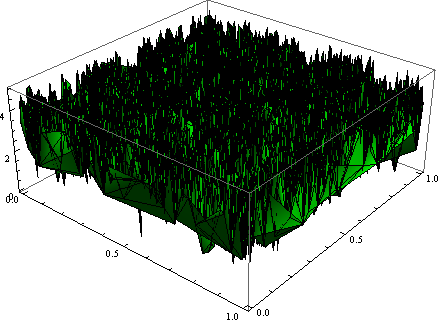
\includegraphics[scale=0.85]{problem1/my/AEE/18}
    \caption{18-та ітерація. Кількість скінченних елементів - 19322}
    \label{fig:p1_aee18}
\end{figure}

З \autoref{fig:p1_aee18} бачимо, що отримане розбиття характеризується, тим що похибка розділена майже рівномірно по всіх скінченних елементах.

Нижче в таблиці наведено числові результати роботи схеми

\pgfplotstabletypeset[col sep=comma,
	columns/0/.style={
		column name=\textnumero
	},
	columns/1/.style={
		column name=$N(h)$
	},
	columns/2/.style={
		column name=$M(h)$
	},
	columns/3/.style={
		column name=$\norm{e_h}^\prime$
	},
	columns/4/.style={
		column name=$\norm{e_h}$
	},
	columns/5/.style={
		column name=$\norm{e}$
	},
	columns/6/.style={
		column name=${P[H_1, u_h]}$
	},
	columns/7/.style={
		column name=$\frac{\norm{e_h}}{\norm{e_h+u_h}}$
	},
%%
	begin table=\begin{longtable},
	end table=\end{longtable},
%
	every head row/.style={before row=\caption{Похибки та збіжність схеми}\\\toprule, after row=\midrule},
	every last row/.style={after row=\bottomrule},
	every nth row={1}{before row=\midrule},
	column type/.add={|}{|}
]{include/8NumResults/problem1/my/errors/table.csv}

Тут
\begin{equation*}
	\begin{split}
		&\norm{e_h^\prime} \text{ - оцінювач представлений в \cite{OstShynAee11} } \\
		&\norm{e_h} \text{ - оцінювач представлений в даній роботі} \\
		&\norm{e} \text{ - реальна похибка} \\
		&P[H_1, u_h]_i = \ln \frac{\ln{e_h^i}-\ln{e_h^{i-1}}}{\ln{N_{i-1}}-\ln{N_h}} \text{ - показник збіжності} \\
	\end{split}
\end{equation*}

Наведемо також графік залежності норми похибок від кількості елементів.

\begin{figure}[H]
	\centering
    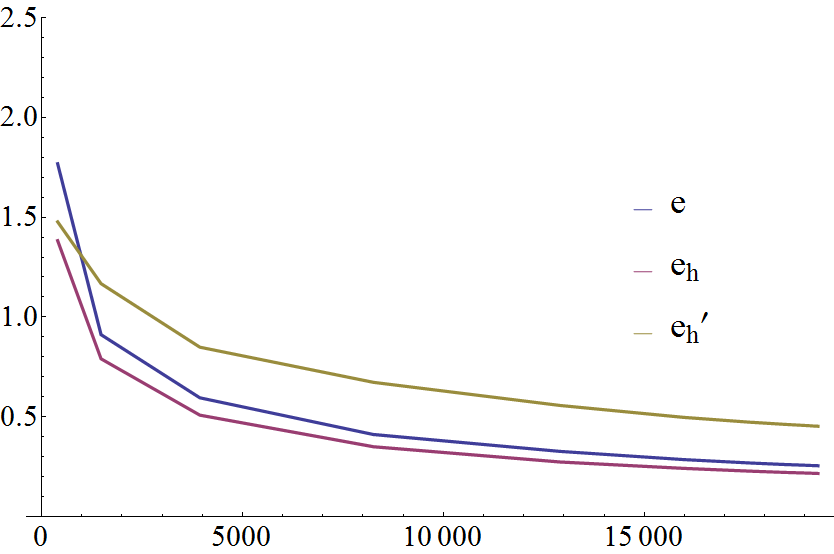
\includegraphics[scale=0.65]{problem1/my/Plotnb}
    \caption{Залежність норм похибок від кількості елементів}
    \label{fig:p1_my_errors}
\end{figure}

Якщо ж за основу для адаптивної стратегії взяти оцінювач з \cite{OstShynAee11}, то таблиця обчислених результатів матиме вигляд.

\pgfplotstabletypeset[col sep=comma,
	columns/0/.style={
		column name=\textnumero
	},
	columns/1/.style={
		column name=$N(h)$
	},
	columns/2/.style={
		column name=$M(h)$
	},
	columns/3/.style={
		column name=$\norm{e_h}^\prime$
	},
	columns/4/.style={
		column name=$\norm{e_h}$
	},
	columns/5/.style={
		column name=$\norm{e}$
	},
	columns/6/.style={
		column name=${P[H_1, u_h]}$
	},
	columns/7/.style={
		column name=$\frac{\norm{e_h}}{\norm{e_h+u_h}}$
	},
%%
	begin table=\begin{longtable},
	end table=\end{longtable},
%
	every head row/.style={before row=\caption{Похибки та збіжність схеми}\\\toprule, after row=\midrule},
	every last row/.style={after row=\bottomrule},
	every nth row={1}{before row=\midrule},
	column type/.add={|}{|}
]{include/8NumResults/problem1/ost/errors/table.csv}

Як бачимо схема доходить до сітки з вдвічі більшою кількістю елементів і незважачи на це знаходить розв'язок з більшою похибкою. Графік залежності похибки від кількості елементів має вигляд.


\begin{figure}[H]
	\centering
    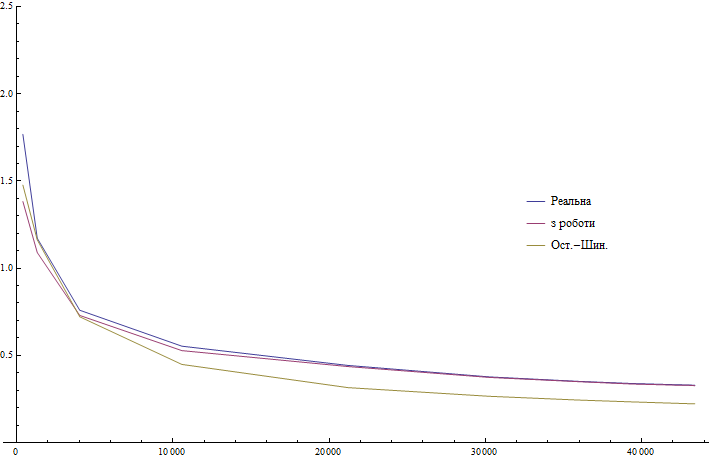
\includegraphics[scale=0.65]{problem1/ost/Plotnb}
    \caption{Залежність норм похибок від кількості елементів}
    \label{fig:p1_ost_errors}
\end{figure}
